\section{Funciones armónicas}
Esta sección tratará de funciones armónicas. En lo que sigue se denotará con $\Omega$ a un dominio de $\mathbb{R}^n$ y $u$ una función $u$ definida como sigue
$$u:\Omega \in \mathbb{R}^n \longrightarrow \mathbb{R}$$

\begin{definition}{Función armónica}
Se dice que $u$ es \textbf{armónica} $\iff u\in C^2(\Omega)$ y $\Delta u = 0$ en $\Omega$.

\noindent Se dice que $u$ es \textbf{subarmónica} $\iff u\in C^2(\Omega)$ y $\Delta u \ge 0$ en $\Omega$.

\noindent Se dice que $u$ es \textbf{superarmónica} $\iff u\in C^2(\Omega)$ y $\Delta u \le 0$ en $\Omega$.
\end{definition}

\subsection{Propiedad del valor de la media}
\begin{mathresult}{Propiedad de la media de las funciones armónicas}
Sea $u$ una función armónica y $B(x,R)$ una bola de centro $x$ y radio $R$. Si $\overline{B(y,R)}\in \Omega$, se tiene que 
$$u(x) = \frac{1}{|\delta B_R(x)|}\int_{\delta B_R} u(x)dS = \frac{1}{|B_R(x)|} \int_{B_R}u(x)dV$$
donde $\omega_n$ es el área de la bola unidad de dimensión $n$. Es decir, estos tres valores son iguales:
\begin{itemize}
\item El valor de la función en el centro de la bola
\item El valor medio de la función en la superficie de la bola.
\item El valor medio en el interior de la bola.
\end{itemize}

Para funciones \textbf{subarmónicas}, se tiene que el valor en el centro de la bola es \textbf{menor o igual} que el promedio de la función.

Para funciones \textbf{superarmónicas}, se tiene que el valor en el centro de la bola es \textbf{mayor o igual} que el promedio de la función.
\end{mathresult}

\begin{proof}
\indent Sea $u$ una función subarmónica e $y\in\Omega$ un punto del dominio $\Omega$ tal que $\exists B_R(y)$, una bola de radio $R$ centrada en $y$ que cumpe que $\overline{B_R(y)}\in\Omega$.
\vspace{5mm}

En primer lugar vamos a definir $\omega_n$ como el área de la superficie bola unitaria de dimensión $n$. Es decir
$$\omega_n = \frac{2\pi^{n/2}}{\Gamma(n/2)}$$ De esta manera, el volumen de la misma bola será $\omega_n/n$.
Realizando un simple cambio de variable, se obtiene que el área de la superficie de la bola de radio $R$ de dimensión $n$ es $\omega_nR^{n-1}$ y su volumen $\frac{R^n\omega_n}{n}$.

En resumen:
\begin{equation*}
\left\{
\begin{array}{l}
\text{Área}(\delta B_1) = \omega_n\\
\text{Vol}(B_1) = \frac{\omega_n}{n}\\
\text{Área}(\delta B_R) = \omega_nR^{n-1}\\
\text{Vol}(B_R) = \frac{R^n\omega_n}{n}
\end{array}
\right.
\end{equation*}

Consideramos
$$g(\rho) = \frac{1}{|\delta B_\rho|}\int_{\delta B_\rho(y)} u(\xi)dS_\xi = \frac{1}{\omega_n \rho^{n-1}}\int_{\delta B_\rho(y)} u(\xi)dS_\xi$$ para un $\rho \in (0,R)$.

Realizamos ahora un cambio de variable para llevar el resultado a la bola unidad.
\begin{equation*}
\left\{
\begin{array}{l}
\xi = y+\rho w\\
w = \frac{\xi-y}{\rho}\\
|w| = 1
\end{array}
\right.
\end{equation*}
Se tiene
$$g(\rho) = \frac{1}{\omega_n \rho^{n-1}}\int_{\delta B_\rho(y)} u(\xi)dS_\xi = \frac{\rho^{n-1}}{\omega_n \rho^{n-1}}\int_{\delta B_1(y)} u(y+\rho w)dS_w$$
Tomamos ahora 
$$g'(\rho) = \frac{1}{\omega_n}\int_{\delta B_1(y)} \nabla u(y+\rho w)wdS_w$$
Definimos $v(y)$ de forma que cumpla:
\begin{equation*}
\left\{
\begin{array}{l}
v(w) = u(y+\rho w)\\
\nabla v(w) = \nabla u(y+\rho w)\rho\\
\Delta v(y) = \rho^2\Delta u(y+\rho w)
\end{array}
\right.
\end{equation*}
por tanto 
$$g'(\rho) =  \frac{1}{\omega_n}\int_{\delta B_1(y)} \frac{1}{\rho} \nabla v(w)wdS_w =  \frac{1}{\omega_n \rho}\int_{\delta B_1(y)} <\nabla v(w), w>dS_w$$
usando el teorema de la divergencia
$$g'(\rho) =  \frac{1}{\omega_n \rho}\int_{B_1(y)} \Delta v(w)dS_w = 0$$
Si $g'(\rho) = 0\implies g(\rho) = cte$ en $(0,R)$. Como $u$ es continua, $g(\rho) = u(y)$.

$$u(y) = \frac{1}{|\delta B_\rho(y)|}\int_{\delta B_\rho(y)}u(\xi)dS_\xi$$
lo que ocurre $\forall \rho \in (0,R)$

Por otro lado, si lo anterior se integra en $(0,R)$
$$\int_0^R u(y) d\rho = \frac{R^n}{n}u(y) = \frac{1}{\omega_n} \int_0^R d\rho \int_{\delta B_\rho(y)} u (\xi) dS_\xi = \frac{1}{\omega_n}\int_{B_R(y)} u(x) dx$$
Luego 
$$u(y) = \frac{n}{\omega_n R^n}\int_{B_R(y)} u(x) dx = \frac{1}{|B_R(y)|} \int_{B_R(y)} u(x) dx$$
\end{proof}


\begin{mathresult}{Principio fuerte del máximo para funciones subarmónicas}
Sea $u(x)$ una función armónica en $\Omega$. Si $u$ alcanza su máximo en $\Omega$, entonces $u$ es constante en $\Omega$.
\end{mathresult}
\begin{proof}
Sea $M=\sup_\Omega u$ y $\Omega_M = \{x\in\Omega: u(x) = M\}$. Está claro que $\Omega_M$ es cerrado relativo a $\Omega$. Vamos a demostrar que $\Omega_M$ es también un abierto relativo a $\Omega$. De esta forma, como $\Omega$ es un dominio, al ser conexo, los únicos subconjuntos que son simultáneamente abiertos y cerrados son el vacío y el propio $\Omega$. Si $u$ tiene un máximo en $x_0$, tendríamos que $x_0\in\Omega_M\neq\emptyset$. Luego, $\Omega_M = \Omega$.

Sea $z\in\Omega_M$. Tenemos
$$0=(u(z) - M) = \frac{1}{|B_R|}\int_{B_R}(u(x)-M)dx = \frac{1}{|B_R|}\int_{B_R} 0dx = 0$$
Es decir, tenemos que $u(x)-M = 0$ en toda la bola. Por lo que para todo $z\in\Omega_M$ podemos encontrar una bola $B$ abierta tal que $B\in\Omega_M$, luego $\Omega_M$ es abierto.
\end{proof}

\subsection{Solución del problema de Dirichlet para el disco unidad}
\noindent De aquí en adelante, se denotará
$$\mathbb{D} = \{(x,y)\in \mathbb{R}^2: x^2+y^2 < 1\}$$
Dada $f\in\delta\mathbb{D}$, continua, $2\pi-$periódica y definida como sigue:
$$f:\mathbb{R}\longrightarrow\mathbb{R}$$
se quiere encontrar $u\in C^2(\mathbb{D})\cap C(\mathbb{\overline{\mathbb{D}}})$ que satisfaga
\begin{equation*}
\left\{
\begin{array}{l l}
-\Delta u = 0 & \text{en } \mathbb{D}\\
u=f & \text{en } \delta\mathbb{D}
\end{array}
\right.
\end{equation*}
Las soluciones que buscamos tienen la forma
$$u(x,y) = R(r)T(\theta)$$
con $r=||(x,y)||=\sqrt{x^2+y^2}$
Dado que la función $u$, es armónica, $u$ verifica $\Delta u = 0$, o lo que es lo mismo
$$R''T+\frac{1}{r}R'T+\frac{1}{r^2}RT'' = 0$$
Separando las variables, se obtiene
$$\frac{r^2R''+rR'}{R}=\frac{-T''}{T}$$
Observamos que tenemos una igualdad de dos funciones que dependen de variables distintas. El primer término depende sólamente de $r$, mientras que el segundo depende de $\theta$. Esto implica que dichos términos han de ser iguales a una constante $\lambda$, luego se tiene que
\begin{align}\label{eq:dirich1}
r^2R''+rR'-\lambda r = 0\\\label{eq:dirich2}
T''+\lambda T = 0
\end{align}
Tenemos un sistema de dos EDOs independientes, la primera es la ecuación de Cauchy-Euler, y la segunda es sencilla de resolver.
Las posibles soluciones para ambas EDOs son:
\begin{equation*}
\eqref{eq:dirich1}\ R(r) = \left\{
\begin{array}{l l}
1,log(r) & \lambda=0\\
r^{\sqrt{\lambda}}, r^{-\sqrt{\lambda}} & \lambda > 0\\
\text{soluciones complejas} & \lambda < 0
\end{array}
\right.
\end{equation*}
\begin{equation*}
\eqref{eq:dirich2}\ T(\theta) = \left\{
\begin{array}{l l}
1,\theta & \lambda=0\\
cos(\sqrt{\lambda}\theta), sin(\sqrt{\lambda}\theta) & \lambda > 0\\
cosh(\sqrt{-\lambda\theta}), sinh(\sqrt{-\lambda\theta}) & \lambda < 0
\end{array}
\right.
\end{equation*}
No se puede suponer que para todos los valores de $\lambda$ y para toda elección de $R$ y $T$, la fórmula $u(x,y) = R(r)T(\theta)$ va a definir una función armónica en un dominio $\Omega$. Esto es sólo verdad si se define una función $C^2(\Omega)$. Si $\Omega$ contiene curvas que encierran al origen, entonces la función $u$ será $2\pi-$periódica. En este caso $\Omega=\mathbb{D}$, por lo que $u$ ha de ser $2\pi-$periódica.

\noindent Eliminamos las siguientes soluciones por no ser $2\pi-$periódicas.
\begin{equation*}
\eqref{eq:dirich2}\ T(\theta) = \left\{
\begin{array}{l l}
1,\color{red}{\theta} & \lambda=0\\
cos(\sqrt{\lambda}\theta), sin(\sqrt{\lambda}\theta) & \lambda > 0\\
\color{red}{cosh(\sqrt{-\lambda\theta})}, \color{red}{sinh(\sqrt{-\lambda\theta})} & \lambda < 0
\end{array}
\right.
\end{equation*}
Para que
\begin{equation*}
\left.
\begin{array}{l l}
cos(\sqrt{\lambda}(\theta+2\pi)) = cos(\sqrt{\lambda}(\theta))\\
sin(\sqrt{\lambda}(\theta+2\pi)) = sin(\sqrt{\lambda}(\theta))\\
\end{array}
\right\} \iff \lambda = n^2
\end{equation*}
con $n=1,2,3,\hdots$

\noindent Eliminamos las siguientes soluciones dado que $(0,0)\in\mathbb{D}$
\begin{equation*}
\eqref{eq:dirich1}\ R(r) = \left\{
\begin{array}{l l}
1,\color{red}{log(r)} & \lambda=0\\
r^{\sqrt{\lambda}}, \color{red}{r^{-\sqrt{\lambda}}} & \lambda > 0\\
\end{array}
\right.
\end{equation*}
Se tiene entonces que $u$ es combinación lineal de las soluciones anteriores (tomamos la constante como $\frac{a_0}{2}$ por comodidad):
$$u_N(x,y) = \frac{a_0}{2}+\sum_{n=1}^Nr^n(a_ncos(n\theta)+b_nsin(n\theta))$$
La condición de frontera del problema de Dirichlet pide que $u=f$ en $\delta\Omega$. Por tanto
$$U_N(1,\theta) = f(\theta)$$
Si $f$ se puede escribir como combinación lineal de senos y cosenos, entonces el problema tiene solución y como ya se ha visto, dicha solución es única.
Supongamos que
$$f(\theta) = \frac{a_0}{2} + \sum_{n=1}^\infty (a_ncos(n\theta)+b_nsin(n\theta))$$
Se puede observar (ver figura \ref{fig:int-period}) que
\begin{equation*}
\int_0^{2\pi} cos(n\theta)d\theta = \int_0^{2\pi} sin(n\theta)d\theta=0
\end{equation*}
\begin{figure}[ht]
	\centering
	\begin{subfigure}{.5\textwidth}
	\centering
	\begin{tikzpicture}
	    \fill[fill=lavenderblue, samples=400, scale=0.5] (0,0) -- plot [domain=0:2*pi] (\x,{sin(4*(\x r))}) -- (2*pi,0) -- cycle;
    	\draw plot[domain=0:2*pi, samples=400, scale=0.5] (\x,{sin(4*(\x r))});
	    \draw[->] (-0.3,0) -- (pi+0.3,0);
	    \draw[->] (0,-0.3) -- (0,1.3);
	\end{tikzpicture}
	\caption{$sin(n\theta)$}
	\end{subfigure}%
	%
	\begin{subfigure}{.5\textwidth}
	\centering
	\begin{tikzpicture}
	    \fill[fill=lavenderblue, samples=400, scale=0.5] (0,0) -- plot [domain=0:2*pi] (\x,{cos(4*(\x r))}) -- (2*pi,0) -- cycle;
    	\draw plot[domain=0:2*pi, samples=400, scale=0.5] (\x,{cos(4*(\x r))});
	    \draw[->] (-0.3,0) -- (pi+0.3,0);
	    \draw[->] (0,-0.3) -- (0,1.3);
	\end{tikzpicture}
	\caption{$cos(n\theta)$}
	\end{subfigure}
	\caption{Integrales periódicas}
	\label{fig:int-period}
\end{figure}
Luego
$$\int_0^{2\pi} f(\theta)d\theta = \frac{a_0}{2}2\pi+0$$
obteniéndose así
$$\frac{a_0}{2} = \frac{1}{2\pi}\int_0^{\pi}f(\theta)d\theta$$
Ahora vamos a ver los valores que toman $a_n$ y $b_n$ para cada valor de $n$.
\begin{itemize}
\item Valor de $a_n$
\begin{align*}
\int_0^{2\pi}f(\theta)cos(m\theta)d\theta = & \frac{a_0}{2}\underbrace{\int_0^{2\pi}cos(m\theta)}_{=0} +\\
+ & \sum_{n=1}^\infty\left(a_n\underbrace{\int_0^{2\pi}cos(n\theta)cos(m\theta)d\theta}_{=\pi}\right) +\\
+ & \sum_{n=1}^\infty\left(b_n\underbrace{\int_0^{2\pi}sin(n\theta)cos(m\theta)d\theta}_{=0}\right)
\end{align*}
Luego
$$a_m = \frac{1}{\pi}\int_0^{2\pi}f(\theta)cos(m\theta)d\theta$$
\item Valor de $b_n$
\begin{align*}
\int_0^{2\pi}f(\theta)sin(m\theta)d\theta = & \frac{a_0}{2}\underbrace{\int_0^{2\pi}sin(m\theta)}_{=0} +\\
+ & \sum_{n=1}^\infty\left(a_n\underbrace{\int_0^{2\pi}cos(n\theta)sin(m\theta)d\theta}_{=0}\right) +\\
+ & \sum_{n=1}^\infty\left(b_n\underbrace{\int_0^{2\pi}sin(n\theta)sin(m\theta)d\theta}_{=\pi}\right)
\end{align*}
Luego
$$b_m = \frac{1}{\pi}\int_0^{2\pi}f(\theta)sin(m\theta)d\theta$$
\end{itemize}
Tenemos entonces que $u$ es de la forma
\begin{align*}
u(r,\theta) = & \frac{a_0}{2}+\sum_{n=1}^\infty r^n\left(a_ncos(n\theta)+b_n sin(n\theta)\right) =\\
= & \frac{1}{2\pi}\int_0^{2\pi}f(\theta)d\theta+\\
+ & \sum_{n=1}^\infty r^n\left(\frac{1}{\pi}\int_0^{2\pi}f(\varphi)cos(n\varphi)d\varphi cos(n\theta)\right) + \\
+ & \sum_{n=1}^\infty r^n\left(\frac{1}{\pi}\int_0^{2\pi}f(\varphi)sin(n\varphi)d\varphi sin(n\theta)\right) = \\
= & \frac{1}{\pi}\int_0^{2\pi}f(\varphi)\left\{\frac{1}{2}+\sum_{n=1}^\infty r^n\left(cos(n\varphi)cos(n\theta)+sin(n\varphi)sin(n\theta)\right)\right\}d\varphi = \\
= & \frac{1}{\pi}\int_0^{2\pi}f(\varphi)\left\{\frac{1}{2}+\sum_{n=1}^\infty r^n\left(cos(n(\theta-\varphi))\right)\right\}d\varphi 
\end{align*}
En definitiva:
$$u(r,\theta) = \int_0^{2\pi}f(\varphi)P(r,\theta-\varphi)d\varphi$$
donde
$$P(r,\varphi)=\frac{1}{\pi}\left\{\frac{1}{2}+\sum_{n=1}^\infty r^n cos(n\varphi)\right\}$$
Vamos a calcular el valor de $P(r, \varphi)$. Sea $z=re^{i\varphi}$. Se tiene que $z^n=r^ne^{in\varphi}$. Si $|z|<1$, se tiene que
$$\sum_{n=1}^\infty z^n = \frac{z}{1-z}$$
Así que 
$$\sum_{n=1}^\infty z^n + \frac{1}{2} = \frac{1+z}{2(1-z)}$$
Entonces
$$P(r,\varphi) = \frac{1}{2\pi}Re\left(\frac{1+z}{1-z}\right)$$
Vamos a simplificar este valor, multiplicando el numerador y el denominador por el conjugado de $1-z$.
$$\frac{1+z}{1-z}\cdot\frac{1-\overline{z}}{1-\overline{z}} = \frac{1-r^2+(z-\overline{z})}{|1-\overline{z}|^2} = \frac{1-r^2-2iIm(z)}{1+r^2-2Re(z)}$$
De donde se obtiene la parte real de $\frac{1+z}{1-z}$
$$P(r,\varphi) = \frac{1}{2\pi}\cdot\frac{1-r^2}{1-2rcos(\varphi)+r^2}$$
\begin{mathresult}{Solución del problema de Dirichlet}
La solución del problema de Dirichlet en el disco unidad es de la forma $$u(r,\theta) = \int_0^{2\pi}f(\varphi)P(r,\theta-\varphi)d\varphi$$
donde $P(r, \varphi)$ es el núcleo de Poisson.
$$P(r,\varphi) = \frac{1}{2\pi}\cdot\frac{1-r^2}{1-2rcos(\varphi)+r^2}$$
\end{mathresult}
\subsubsection{Núcleo de Poisson}
Como ya se ha visto, el \textbf{núcleo de Poisson} tiene la forma $$P(r,\varphi) = \frac{1}{2\pi}\cdot\frac{1-r^2}{1-2rcos(\varphi)+r^2}$$
Veamos unas pocas propiedades de esta función
\begin{itemize}
\item \textbf{Definición}

\begin{equation*}
\text{El núcleo de Poisson está definido en}
\left\{
\begin{array}{l}
0\le r\le 1\\
\varphi \neq 0
\end{array}
\right.
\text{ver figura \ref{fig:def-poisson}.}
\end{equation*}

\begin{figure}[ht]
\centering
\begin{tikzpicture}[scale=1.5]
	\draw[->] (-1.5,0) -- (1.5,0) node[right] {$x$};
	\draw[->] (0,-1.5) -- (0,1.5) node[above] {$y$};
	\draw [fill, lavenderblue] (0,0) circle [radius=1];
	\draw [] (0,0) circle [radius=1];
	\draw [fill, white] (1,0) circle [radius=0.07];
	\draw [] (1,0) circle [radius=0.07];
	\node (0,0) {$\mathbb{D}$};
\end{tikzpicture}
\caption{Dominio del núcleo de Poisson}
\label{fig:def-poisson}
\end{figure}

\item $P(r, \varphi)$ \textbf{es armónica}
Dado que $u(r,\theta)$ es armónica y 
$$u(r,\theta)=\int_0^{2\pi}f(\varphi)P(r,\theta-\varphi)d\varphi$$
Se tiene que 
$$0 = \Delta u(r,\theta)=\int_0^{2\pi}f(\varphi)\Delta P(r,\theta-\varphi)d\varphi$$
Es decir
$$\Delta P(r,\theta) = 0$$

\item $\int_0^{2\pi}P(r,\varphi)d\varphi = 1$

Basta tomar $f(\theta) = 1$ y comprobar que $u=1$ es solución. Por tanto
$$u(r, \theta) = 1 = \int_0^{2\pi}1\cdot P(r,\theta-\varphi)d\varphi$$

\item $\int_{-\pi}^{\pi}P(r,\varphi)d\varphi = 1$

Dado que las integrales necesarias para calcular lo anterior tienen el mismo valor entre $-\pi$ y $\pi$, basta repetir la prueba anterior.
\end{itemize}

\begin{theorem}

Si $f$ es continua en $\theta_0$, entonces
$$\lim_{(r,\theta)\to(1,\theta_0)}=f(\theta_0)$$
\end{theorem}
\begin{proof}
Vamos a calcular
$$u(r,\theta)-f(\theta_0)$$
Dado que $$\int_{-\pi}^{\pi}P(r,\tilde{\varphi})d\tilde{\varphi} = 1$$
Se tiene que 
$$u(r,\theta)-f(\theta_0)\cdot 1 = u(r,\theta)-f(\theta_0)\int_{-\pi}^{\pi}P(r,\tilde{\varphi})d\tilde{\varphi}$$
Si realizamos el siguiente cambio de variable:
\begin{equation*}
\left.
\begin{array}{l}
\tilde{\varphi} = \theta+\varphi\\
d\tilde{\varphi} = d\varphi
\end{array}
\right\}
\end{equation*}
entonces
$$u(r,\theta)-f(\theta_0)\int_{-\pi}^{\pi}P(r,\tilde{\varphi})d\tilde{\varphi}=\frac{1-r^2}{2\pi}\int_{-\pi}^{\pi}\frac{f(\theta_0+\varphi)-f(\theta_0)}{1-2rcos(\theta-\theta_0-\varphi)+r^2}$$
Podemos separar lo anterior en tres integrales
$$u(r,\theta)-f(\theta_0)=\frac{1-r^2}{2\pi}\left(\int_{-\pi}^{-\delta}\int_{-\delta}^{\delta}\int_{\delta}^{\pi}\right)\left(\frac{f(\theta_0+\varphi)-f(\theta_0)}{1-2rcos(\theta-\theta_0-\varphi)+r^2}\right)$$
La continuidad de $f$ nos dice que dado un $\varepsilon>0, \exists\delta$ tal que
$$|\varphi|<\delta \implies |f(\theta+\varphi)-f(\theta_0)| < \frac{\varepsilon}{2}$$
Vamos a calcular la integral del medio:
\begin{align*}
\frac{1-r^2}{2\pi}\int_{-\delta}^{\delta}\left(\frac{f(\theta_0+\varphi)-f(\theta_0)}{1-2rcos(\theta-\theta_0-\varphi)+r^2}\right) & \le \\
\frac{1-r^2}{2\pi}\int_{-\delta}^{\delta}\left(\frac{\varepsilon/2}{1-2rcos(\theta-\theta_0-\varphi)+r^2}\right) & =
\frac{\varepsilon}{2}\int_{-\delta}^{\delta}\left(P(r,\varphi)d\varphi\right) = \frac{\varepsilon}{2}\\
\end{align*}
Manteniendo el valor de $\delta$ fijo, si $|\varphi| > \delta$ y $|\theta-\theta_0|<\frac{\delta}{2}$, se tiene que
$$|\theta-\theta_0-\varphi| \ge |\varphi|-|\theta-\theta_0|>\delta-\frac{\delta}{2} = \frac{\delta}{2}$$
Calculamos las otras dos integrales, tomando $M=\max_{\delta\mathbb{D}}f$
\begin{align*}
\frac{1-r^2}{2\pi}\left(\int_{-\pi}^{-\delta}\int_{-\delta}^{\delta}\int_{\delta}^{\pi}\right)\left(\frac{f(\theta_0+\varphi)-f(\theta_0)}{1-2rcos(\theta-\theta_0-\varphi)+r^2}\right)\le \\
\le \frac{2M}{2\pi}\cdot\frac{1-r^2}{1-2rcos(\theta-\theta_0-\varphi)+r^2}\cdot 2(\pi-\delta)\to 0
\end{align*}
si $r\to 1$.
Tenemos por tanto que
$$u(r,\theta)-f(\theta_0) \le \frac{\varepsilon}{2} + \frac{\varepsilon}{2} = \varepsilon$$
\end{proof}

\subsection{Fórmula de representación}
Vamos a buscar soluciones radiales para $\Delta u = 0$ en $\mathbb{R}^n$, lo que quiere decir que buscamos $f(r)$ tal que
$$u(x) = f(r)$$ con $r=||x||$

En primer lugar vamos a hallar el laplaciano en función de $r$.

\begin{equation*}
\begin{array}{l l l}
\frac{du(x)}{dx_i} & = & f'(r)\frac{x_i}{r}\\
\frac{d^2u(x)}{dx_i^2} & = & f''(r)\frac{x_i^2}{r^2}+f'(r)\frac{r^2-x_i\frac{x_i}{r}}{r^2}\\
& = & f''(r)\frac{x_i^2}{r^2}+f'(r)\frac{r^2-x_i^2}{r^3}\\
\Delta u(x) & = & \sum_{i=0}^N\frac{d^2u(x)}{dx_i^2} = f''(r)+f'(r)\frac{N-1}{r} = \frac{1}{r^{N-1}}\left(r^{N-1}f'(r)\right)'
\end{array}
\end{equation*}

Vamos a calcular soluciones radiales para
\begin{equation*}
\left\{
\begin{array}{l l}
\Delta u(x) = 0 & \text{en } \mathbb{R}^n\\
u(x) = f(r)
\end{array}
\right.
\end{equation*}
Como $\Delta u(x) = \frac{1}{r^{N-1}}\left(r^{N-1}f'(r)\right)'$ y $\Delta u(x) = 0$. Se tiene que $\left(r^{N-1}f'(r)\right)$ es constante
$$r^{N-1}f'(r) = A$$ de donde se obtiene
$$f(r) = \frac{A}{N-2}\cdot \frac{1}{r^{N-2}} + B$$ con $A,B$ constantes.

Si $u(x) = 1$, tenemos que la solución es 
$\Gamma(x) = \frac{1}{r^{N-2}} = \frac{1}{||x||^{N-2}}$ para $N\neq 2$ y $\Gamma(x) = log(r)$ para $N=2$. En cualquier caso se cumple que $\Delta\Gamma(x) = 0$ en $\mathbb{R}^N\setminus\{ 0 \}$

En lo que sigue vamos a tener presente las siguientes equivalencias
\begin{equation*}
\begin{array}{l}
\Delta u = div \nabla u = \nabla^2 u\\
div(f\cdot F) = f\cdot div(F)+div(f)\cdot F
\end{array}
\end{equation*}
De esta forma, se cumplen las igualdades que siguen:
\begin{equation*}
\left\{
\begin{array}{l}
div(v\nabla u)=v\Delta u+\nabla v\nabla u\\
div(u\nabla v)=u\delta v+\nabla u\nabla v\\
\end{array}
\right.
div(v\nabla u-u\nabla v) = v\Delta u-u\Delta v
\end{equation*}
Sea $y\in \Omega$ un punto tal que $\exists B_\varepsilon(y)$, una bola $B$ de radio $\varepsilon$ que cumple $\overline{B_\varepsilon(y)}\in\Omega$. Definimos
$$\Omega_\varepsilon = \Omega\setminus \overline{B_\varepsilon(y)}$$
Consideramos ahora 
$$\int_{\Omega_\varepsilon} \left(v\Delta u-u\Delta v\right)dx =\int_{\Omega_\varepsilon} div\left(v\nabla u-u\nabla v\right)dx $$
Utilizando el teorema de la divergencia
$$\int_{\Omega_\varepsilon} div\left(v\nabla u-u\nabla v\right)dx =\int_{\delta\Omega_\varepsilon} \left(v\frac{du}{d\nu}-u\frac{dv}{d\nu}\right)d\xi$$
con $\nu$ la normal exterior a $\delta\Omega_\varepsilon$.

Tomamos $v(x) = \Gamma(x-y)$ que como ya hemos visto cumple que $\Delta v(x) = 0$ en $\mathbb{R}^N\setminus\{y\}$.

Utilizando el resultado anterior y que $\delta \Omega_\varepsilon = \delta\Omega \cup \delta B_\varepsilon(y)$ 
\begin{align*}
& \int_{\Omega_\varepsilon} \frac{1}{|x-y|^{N-2}}\Delta u(x)dx =\\
& \int_{\delta\Omega_\varepsilon} \left(\frac{1}{|\xi-y|^{N-2}}\frac{du(\xi)}{d\nu}-u(\xi)\frac{d}{d\nu}\left(\frac{1}{|\xi-y|^{N-2}}\right)\right)dS_\xi \ + \\
& \int_{\delta B_\varepsilon(y)} \left(\frac{1}{\varepsilon^{N-2}}\frac{du(\xi)}{d\nu}-u(\xi)\frac{d}{d\nu}\left(\frac{1}{|\xi-y|^{N-2}}\right)\right)dS_\xi\\
\end{align*}

Vamos a estudiar ambos términos por separado. Sea $M=\max_{\overline{\Omega}}|\nabla u(x)|$, como $u\in C^2(\Omega)\cup C^1(\overline{\Omega})$, si $\varepsilon\to 0$
\begin{align*}
& \int_{\delta B_\varepsilon(y)} \left(\frac{1}{\varepsilon^{N-2}}\frac{du(\xi)}{d\nu}-u(\xi)\frac{d}{d\nu}\left(\frac{1}{|\xi-y|^{N-2}}\right)\right)dS_\xi \ \le\\
& \frac{1}{\varepsilon}M\int_{\delta B_\varepsilon(y)} dS_\varepsilon \ = \frac{1}{\varepsilon^{N-2}}M|\delta B_\varepsilon| \ = M\omega_n\varepsilon\to 0\\
\end{align*}

En $\delta B_\varepsilon$ tenemos que $\nu = \frac{\xi-y}{\varepsilon}$ por tanto, si $\varepsilon\to0$
$$\frac{d}{d\nu}\left(\frac{1}{|\xi-y|^{N-2}}\right) = -\left.\frac{d}{dr}\right|_{r=\varepsilon}\frac{1}{r^{N-2}} = (N-2)\varepsilon^{1-N}$$ si tomamos $r=|\xi-y|$. Luego
\begin{align*}
& \int_{\delta B_\varepsilon} u(\xi)\frac{d}{d\nu}\left(\frac{1}{|\xi-y|^{N-2}}\right)dS_\xi \ = (N-2)\varepsilon^{1-N}\int_{\delta B_\varepsilon}u(\xi)dS_\xi \ = \\
& (N-2)\varepsilon^{1-N}\varepsilon^{N-1}\int_{\delta B_1}u(y+\varepsilon w)dS_\xi\to(N-2)|\delta B_1|u(y)
\end{align*}

Nos queda que 
\begin{align*}
|N-2||\delta B_1|u(y) = & -\int_{\Omega}\frac{\Delta u(x)}{|x-y|^{N-2}}dx\\
& + \int_{\delta\Omega} \frac{1}{|\xi-y|^{N-2}}\cdot\frac{du(\xi)}{d\nu}dS_\xi\\
& -\int_{\delta\Omega}u(\xi)\frac{d}{d\nu}\left(\frac{1}{|\xi-y|^{N-2}}\right)dS_\xi
\end{align*}

Esta fórmula de representación implica que
\begin{equation*}
\left.
\begin{array}{l l}
\Delta u & \text{en } \Omega\\
u & \text{en } \delta\Omega\\
\frac{du}{d\nu} & \text{en } \delta\Omega\\
\end{array}
\right\} \text{determinan } u \text{ en } \Omega
\end{equation*}
Se necesitan conocer tres valores, mientras que en el problema de Dirichlet sólo hemos necesitado los dos primeros. Por ello, vamos a manipular la fórmula para que deje de depender del tercer término. Sea $h(x)$ una función armónica. El teorema de la divergencia dice que
$$\int_{\Omega}h(x)-\Delta u(x) - u(x)\Delta h(x) = \int_{\delta\Omega}\left(h\frac{du}{d\nu}-u\frac{dh}{d\nu}\right)$$
Luego 
$$\int_{\Omega}h(x)-\Delta u(x) - u(x)\Delta h(x) - \int_{\delta\Omega}\left(h\frac{du}{d\nu}-u\frac{dh}{d\nu}\right) = 0$$
Sumar esta diferencia a la fórmula de representación que ya tenemos es como sumarle 0. Por simplicidad de notación, vamos a denotar $G(x,y) = \frac{1}{|x-y|^{N-2}}+h(x)$. Tras realizar la suma:
\begin{align*}
|N-2||\delta B_1|u(y) = & -\int_{\Omega}G(x,y)\Delta u(x)dx\\
& + \int_{\delta\Omega} G(\xi, y)\frac{du(\xi)}{d\nu}dS_\xi\\
& -\int_{\delta\Omega}u(\xi)\frac{dG(\xi, y)}{d\nu}dS_\xi
\end{align*}
Queremos librarnos del segundo término, por lo que hay que elegir $h$ para que $G$\footnote{$G$ se conoce como la función de Green para el dominio $\Omega$} sea $0$ en la frontera de $\Omega$. Tomamos $h(x) = \frac{1}{|\xi-y|^{N-2}}$ con $\xi\in\delta\Omega$. Se cumple que $\Delta G(x,y) = 0 \ \forall x \in R^N\setminus \{y\}$ y que $G(\xi,y) = 0 \ \forall \xi \in \delta \Omega$. Tenemos un problema de Dirichlet en $\Omega\setminus\{y\}$.

\subsection{Núcleo de Poisson N-dimensional}
El núcleo de Poisson $N-$dimensional es la función de Green para el dominio $\Omega=B_r(0)$.
Supongamos que $\Delta u = 0$ en $B_r(0)$, y fijemos $x\in B_r(0)$
La fórmula de representación queda de esta forma:
\begin{align*}
|N-2||\delta B_1|u(x) = & -\int_{\Omega}\overbrace{\frac{\Delta u(x)}{|x-y|^{N-2}}}^{0}dx\\
& + \int_{\delta\Omega} \frac{1}{|\xi-x|^{N-2}}\cdot\frac{du(\xi)}{d\nu}dS_\xi\numberthis\label{eq:repr-dirichlet-formula}\\
& -\int_{\delta\Omega}u(\xi)\frac{d}{d\nu}\left(\frac{1}{|\xi-x|^{N-2}}\right)dS_\xi
\end{align*}
Vamos a definir $x'$ como el simétrico de $x$ respecto de la bola. Dada esta definición de $x'$, tenemos que cumple:
\begin{equation*}
\begin{array}{l}
|x||x'|=R^2\\
x'=\frac{R^2}{|x|^2}x
\end{array}
\end{equation*}
Ahora consideramos
$$v(y) = \frac{1}{|y-x'|^{N-2}}$$ que está definida en $\mathbb{R}^N\setminus\{x\}$ y cumple $\Delta v(y) = 0$ en todo su dominio de definición.
Se tiene que
$$\int_\Omega v\underbrace{\Delta u}_0 -u\underbrace{\Delta v}_0 = \int_{\delta B_r} \left(v\frac{du}{d\nu}-u\frac{dv}{d\nu}\right)dS = 0$$
\begin{figure}[ht]
\centering
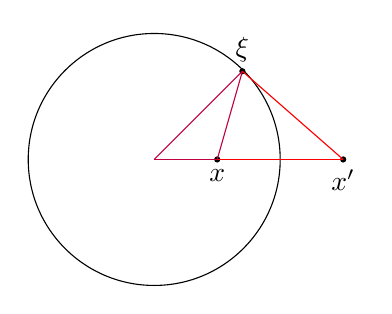
\begin{tikzpicture}[scale=1.6]
\draw[] (0,0) circle[radius=1];
\draw[fill] (0.5,0) circle[radius=0.02] node[below] {$x$};
\draw[fill] (1.5,0) circle[radius=0.02] node[below] {$x'$};
\draw[fill] (0.7,0.7) circle[radius=0.02] node[above] {$\xi$};
\draw[-, purple] (0,0)--(0.5,0);
\draw[-, red] (0.5,0)--(1.5,0);
\draw[-, purple] (0,0)--(0.7,0.7);
\draw[-, purple] (0.5,0)--(0.7,0.7);
\draw[-, red] (1.5,0)--(0.7,0.7);
\end{tikzpicture}
\caption{Dominio $B_r(0)$}
\label{fig: dominiobr}
\end{figure}

Los triángulos $0x\xi$ y $0x'\xi$ son semejantes (ver figura \ref{fig: dominiobr}). Se tiene que
$$\frac{|x|}{R} = \frac{R}{|x'|}$$ Luego $$\frac{|x-\xi|}{|x|} = \frac{|\xi-x'|}{R}$$ es decir, el resto de lados respetan la relación. Todo esto es lo mismo que
$$\frac{1}{|\xi-x|} = \frac{R}{|x|}\cdot\frac{1}{|\xi-x'|}$$
Ya hemos visto que
$$A = \int_{\delta B_r} \left(v\frac{du}{d\nu}-u\frac{dv}{d\nu}\right)dS = 0$$
De donde también se tiene que
$$0 = \left(\frac{R}{|x|}\right)A$$
Luego si a \eqref{eq:repr-dirichlet-formula} le restamos $\left(\frac{R}{|x|}\right)A$ es como si le restáramos $0$.
Nos queda lo siguiente
\begin{align*}
|N-2||\delta B_1|u(x) = \int_{\delta B_r}\left(\overbrace{\frac{1}{|\xi-x|^{N-2}}-\left(\frac{R}{|x|}\right)^{N-2}\frac{1}{|\xi-x'|^{N-2}}}^0\right)\frac{du}{d\nu}dS\\
+ \int_{\delta B_r}u(\xi)\left(\left(\frac{R}{|x|}\right)^{N-2}\frac{d}{d\nu}\left(\frac{1}{|\xi-x'|^{N-2}}\right)-\frac{d}{d\nu}\left(\frac{1}{|\xi-x|^{N-2}}\right)\right)dS
\end{align*}
En $\delta B_R(0)$ se tiene que $\nu=\frac{\xi}{R}$. Luego
$$\frac{d}{d\nu}\left (\frac{1}{|\xi-x'|^{N-2}}\right)=-(N-2)<\frac{\xi}{R}, \frac{\xi-x'}{|\xi-x'|^N}> = \frac{-(N-2)}{R}\cdot\frac{R^2-<\xi,x'>}{|\xi-x'|^N}$$
Y como $x' = \frac{R^2}{|x|^2}x$
$$<\xi,x'> = \frac{R^2}{|x|^2}<\xi, x>$$
Por otro lado
\begin{align*}
\left(\frac{R}{|x|}\right)^{N-2}\frac{d}{d\nu}\left(\frac{1}{|\xi-x'|^{N-2}}\right) =& \frac{-N-2}{R}\left(\frac{R}{|x|}^{N-2}\frac{R^2-\frac{R^2}{|x|^2}<\xi,x>}{|\xi-x'|^N}\right)\\
& = \frac{-N-2}{R}\cdot\frac{|x|^2-<\xi,x>}{|\xi-x'|^N}
\end{align*}
Nos queda, finalmente
\begin{align*}
(N-2)|\delta B_1|u(x) =  \int_{\delta B_R}u(\xi)&\left\{\frac{-N-2}{R}\cdot\frac{|x|^2-<\xi,x>}{|\xi-x|^N}\right. \\
+ & \left.\frac{-N-2}{R}\cdot\frac{R^2-<\xi,x>}{|\xi-x|^N}\right\}dS\\
= \frac{N-2}{R}\int_{\delta B_R}u(\xi)\frac{R^2-|x|^2}{|\xi-x|^n}
\end{align*}
\subsubsection*{Conclusión}
Si $\Delta u(x) = 0$ en $B_R(0)$
$$u(x) = \int_{\delta B_R} u(\xi)P(\xi, x)dS_\xi$$
donde $P(y,x)$ es el núcleo de Poisson $N-$dimensional, definido como sigue:
$$P(y,x) = \frac{R^2-|x|^2}{|\delta B_1| R}\cdot\frac{1}{|y-x|^N}$$
Hemos demostrado el siguiente teorema
\begin{theorem}
Sea $\Omega = B_R(0)$ y $f\in C(\delta B_R)$ y $P(y,x)$ el núcleo de Poisson $N-$dimensional, entonces
$$u(x) = \int_{\delta B_R} f(\xi)P(\xi, x)dS_\xi$$
es la solución del problema de Dirichlet
\begin{equation*}
\left\{
\begin{array}{l l}
-\Delta u = 0 & \text{en } B_R(0)\\
u=f & \text{en } \delta B_R(0)
\end{array}
\right.
\end{equation*}
\end{theorem}

\subsection{Método de separación de variables}
Vamos a ver unos ejemplos
\subsubsection*{Ejemplo 1}
\begin{equation*}
\left\{
\begin{array}{l l}
-\Delta u = 0 & \text{en } \mathbb{D}\\
u=f & \text{en } \delta \mathbb{D}
\end{array}
\right.
\end{equation*}
Dado que $\Delta u$ y $\mathbb{D}$ son invariantes por transformaciones lineales, buscamos una solución de la forma $u(r,\theta)=R(r)T(\theta)$. Como ya hemos visto, la EDP se desacopla en dos EDOs independientes
$$\frac{r^2R''+rR'}{R} = \frac{-T''}{T} = \lambda$$
Vamos a estudiar la segunda, cuya soución ha de ser $2\pi-$periódica. Tenemos un problema de contorno de la siguiente forma: 
\begin{equation*}
\left\{
\begin{array}{l l}
-T''=\lambda T\\
T(0) = T(2\pi)
\end{array}
\right.
\end{equation*}
Este problema no tiene solución para cualquier $\lambda$ por las restricciones impuestas sobre la periodicidad.
Esto es lo que se llama un operador.
\begin{definition}{Operador diferencial}
Un operador diferencial es un par $(\mathcal{L}, P(\mathcal{L}))$ donde $\mathcal{L}$ es un funcional de diferenciación y $P(\mathcal{L})$ el dominio de las funciones.
\end{definition}
En este caso el operador que tenemos es el siguiente
\begin{equation*}
\left\{
\begin{array}{l l}
\mathcal{L}(\varphi) = -\varphi''\\
D(\mathcal{L}) = \{\varphi\in C^2(\mathbb{R}): \phi \text{ es } 2\pi-\text{periódica}\}
\end{array}
\right.
\end{equation*}

\subsubsection*{Ejemplo 2}
\begin{equation*}
\left\{
\begin{array}{l l}
-\Delta u = 0 & \text{en } Q=(0,\pi)\times(0,1)\\
u=h & \text{en } \delta Q
\end{array}
\right.
\end{equation*}
\begin{figure}[ht]
\centering
\begin{tikzpicture}[scale=1.5]
	\draw[->] (-0.5,0) -- (4,0) node[right] {$x$};
	\draw[->] (0,-0.5) -- (0,2) node[above] {$y$};
	\draw[-, thick] (0,0)--(0,1);
	\draw[-, thick] (0,0)--(pi,0);
	\draw[-, thick] (pi,0)--(pi,1);
	\draw[-, thick] (0,1)--(pi,1);
	\draw (0,0.5)  node[left] {$u=0$};
	\draw (pi/2,0)  node[below]{$f(x)$};
	\draw (pi,0.5)  node[right]{$u_x=0$};
	\draw (pi/2,1) node[above] {$g(x)$};
\end{tikzpicture}
\caption{Ejemplo 2}
\label{fig:ej2-sepvar}
\end{figure}
Definamos $h$ como en la figura \ref{fig:ej2-sepvar}.
Buscamos una solución de la forma
$$u(x,y) = X(x)Y(y)$$
El problema vuelve a desacoplarse en dos EDOs independientes
\begin{equation*}
\left\{
\begin{array}{l}
X''=-\lambda X\\
Y'' = \lambda X
\end{array}
\right.
\end{equation*}
Nos fijamos en la primera EDO. Tenemos el operador
\begin{equation*}
\left\{
\begin{array}{l l}
\mathcal{L}(\varphi) = -\varphi''\\
D(\mathcal{L}) = \{\varphi\in C^2(0,\pi)\cap C^1([0,\pi]): \varphi(0) = \varphi'(\pi) = 0\}
\end{array}
\right.
\end{equation*}
Tenemos que 
$$X(x) = Acos(\sqrt{\lambda}x)+Bsin(\sqrt{\lambda}x)$$
Observando los datos iniciales, vemos que $X(0)=0$, luego $A=0$. Por otro lado
$$X'(\pi) = 0 = \sqrt{\lambda}Bcos(\sqrt{\lambda}\pi) \implies cos(\sqrt{\lambda}\pi) = 0 \implies \sqrt{\lambda}\pi = (2n+1)\frac{\pi}{2}$$
Luego $X_n=a_nsin(2n\pi)\frac{\pi x}{2}$
y por tanto $Y_n = A_ncosh(\sqrt{\lambda_n}y)+B_nsinh(\sqrt{\lambda_n}y)$

\subsubsection*{Ejemplo 3}
La ecuación del calor unidimensional es la siguiente
$$u_t-uxx=0$$
donde $t\in\mathbb{R}$ representa el tiempo y $x\in\mathbb{R}$ la posición.
Un posible problema sería colocar una barra de un material cualquiera y estudiar la temperatura de la misma conociendo sólo la distribución inicial de temperaturas y su valor en los extremos.
\begin{equation*}
\left\{
\begin{array}{l l}
u_t-uxx=0 & 0<x<1, t>0\\
u(x,0)=f(x)& \text{Distribución inicial de temperaturas}\\
u(0,t)=u(1,t) = 0 & \text{Temperatura constante en la frontera}
\end{array}
\right.
\end{equation*}

\subsubsection*{Ejemplo 4}
El problema de Neumann es un problema mixto entre un problema de valor inicial y un problema de contorno. Dado que, según las leyes físicas, el flujo de calo es proporcional al gradiente, si se aislan los extremos del problema anterior, se tendría que el flujo de calor es nulo, luego $u_x(0,t)=u_x(1,t) = 0$. El problema quedaría como sigue:
\begin{equation*}
\left\{
\begin{array}{l l}
u_t-uxx=0 & 0<x<1, t>0\\
u(x,0)=f(x)& \text{Distribución inicial de temperaturas}\\
u_x(0,t)=u_x(1,t) = 0 & \text{Extremos aislados}
\end{array}
\right.
\end{equation*}